% *********************************************************************
% © 2026 Jeremy Sylvestre
%
% Permission is granted to copy, distribute and/or modify this document
% under the terms of the GNU Free Documentation License, Version 1.3 or
% any later version published by the Free Software Foundation; with no
% Invariant Sections, no Front-Cover Texts, and no Back-Cover Texts. A
% copy of the license is included in the appendix entitled “GNU Free
% Documentation License” that appears in the output document of this
% PreTeXt source code. All trademarks™ are the registered® marks of
% their respective owners.
%
% *********************************************************************
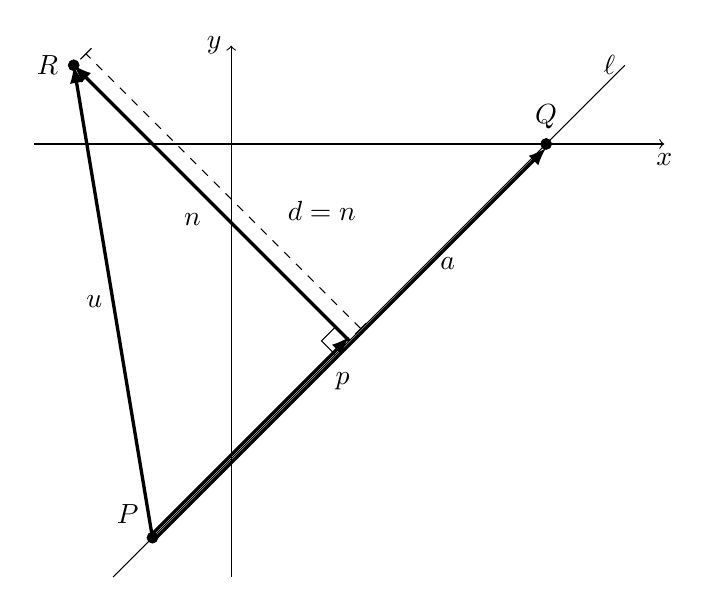
\begin{tikzpicture}[
	vector/.style={-latex,very thick},
	point/.style={circle,draw,very thin,fill,inner sep=0pt,minimum size=4pt},
	% scale=0.75
]
	% projection
	\coordinate (p) at (-1,-5);
	\coordinate (q) at (4,0);
	\coordinate (r) at (-2,1);
	\coordinate (j) at (1.5,-2.5);

	\draw[->] (-2.5,0) to (5.5,0) node[below] {$x$};
	\draw[->] (0,-5.5) to (0,1.25) node[left] {$y$};

	% parallel to (1,1), through (4,0)
	\draw[thin] (-1.5,-5.5) to (5,1) node[left] {$\ell$};

	\node[point] at (p) [label=above left:$P$] {};
	\node[point] at (q) [label=above:$Q$] {};
	\node[point] at (r) [label=left:$R$] {};

	\draw[vector] (p) to node[left] {$\uvec{u}$} (r);
	\draw[vector] ([yshift=-0.05cm]p) to node[below,near end] {$\uvec{a}$} ([yshift=-0.05cm]q);
	\draw[vector] ([yshift=0.05cm]p) to node[below right,very near end] {$\uvec{p}$} ([yshift=0.05cm]j);
	\draw[vector] (j) to node[below left] {$\uvec{n}$} (r);
	\draw[dashed,|-|] ([xshift=0.15cm,yshift=0.15cm]j) to node[xshift=1.25cm,yshift=-0.25cm] {$d = \unorm{n}$} ([xshift=0.15cm,yshift=0.15cm]r);

	% perp symbol
	\begin{scope}[xshift=1.5cm,yshift=-2.5cm]
		\draw[thin,rotate=45] (-0.25,0) to (-0.25,0.25) to (0,0.25);
	\end{scope}

\end{tikzpicture}
